\section{Invariant Manifolds}
Dynamically unstable periodic orbits in the CR3BP have useful structures called invariant manifolds
that represent the local flow near the orbit. With applications for transfer design, trajectories
along these manifold surfaces can be used to arrive at or depart from the periodic orbit
ballistically. Perko provides the following theorem for stable/unstable manifolds for periodic
orbits\cite{Perko:1991}:
\begin{quote}
    Let $f\in C^{1}(E)$ where E is an open subset of $R^{n}$ containing a periodic orbit,
    \begin{equation}
        \Gamma:\xbar=\gamma(t),
    \end{equation}
    of $\xbardot=f(\xbar)$ of period $T$. Let $\phi_{t}$ be the flow of $\xbardot=f(\xbar)$ and
    $\gamma(t)=\phi_{t}(\xbar_{0})$. If $k$ of the characteristic exponents of $\gamma(t)$ have
    negative real part where $0\leq k\leq n-1$ and $n-k-1$ of them have positive real part then
    there is a $\delta>0$ such that the stable manifold of $\Gamma$,
    \begin{equation}
        S(\Gamma)=\{\xbar\in N_{\delta}(\Gamma)|d(\phi_{t}(\xbar),\Gamma)\rightarrow0\text{ as }t\rightarrow\infty\text{ and }\phi_{t}(\xbar)\in N_{\delta}(\Gamma)\text{ for }t\geq0\},
    \end{equation}
    is a $(k+1)$-dimensional, differentiable manifold which is positively invariant under the flow
    $\phi_{t}$ and the unstable manifold of $\Gamma$,
    \begin{equation}
        U(\Gamma)=\{\xbar\in N_{\delta}(\Gamma)|d(\phi_{t}(\xbar),\Gamma)\rightarrow0\text{ as }t\rightarrow-\infty\text{ and }\phi_{t}(\xbar)\in N_{\delta}(\Gamma)\text{ for }t\leq0\},
    \end{equation}
    is an $(n-k)$-dimensional, differentiable manifold which is negatively invariant under the flow
    $\phi_{t}$. Furthermore, the stable and unstable manifolds of $\Gamma$ intersect transversally
    in $\Gamma$.
\end{quote}
In layman's terms, if a periodic orbit is unstable (has eigenvalues greater than and lesser than
$1$), then stable/unstable manifold surfaces exist that approach/leave the orbit asymptotically in
forward time.

Since these manifold structures asymptotically depart the orbit structure, no deterministic
maneuver is required to transfer onto them. However, a consequence of this is that it is not
possible to identify the exact location along the orbit from where a manifold trajectory departs.
Therefore, a numerical process is necessary to approximate the stable/unstable subspace of the
orbit to determine an appropriate initial condition for an arc along the manifold surface.

Near the periodic orbit, the manifolds are tangent to their corresponding eigenspaces of the orbit.
For a selected point on the periodic orbit:
\begin{equation}
    \nubar(t_{0}+t)=\Phi(t_{0}+t,t_{0})\nubar(t_{0}),
    \label{eq:eigenvector}
\end{equation}
where $\nubar(t_{0})$ is the eigenvector at the initial condition corresponding to the stable or
unstable eigenvalue of the monodromy matrix. Once the stable/unstable eigenvector at the selected
point has been obtained:
\begin{equation}
    \nubar_{n}=\frac{\nubar}{\sqrt{\nu_{x}^{2}+\nu_{y}^{2}+\nu_{z}^{2}}},
    \label{eq:normeigenvector}
\end{equation}
where $\nu_{x}$ is the $x$-component of the eigenvector and $\nubar_{n}$ is the eigenvector
normalized by the nondimensional distance from the selected point. Using the normalized
stable eigenvector to approximate the initial condition for a stable manifold arc:
\begin{equation}
    \qbar^{S}=\qbar_{\Gamma}\pm d\nubar_{n}^{S},
    \label{eq:stablemanifold}
\end{equation}
where $\qbar_{\Gamma}$ is the state vector at the selected point along the periodic orbit and $d$
is a step-off distance, generally chosen based on the specific CR3BP system. The scaled eigenvector
can be either added to or subtracted from the periodic state as the eigenspace is bi-directional,
creating two half-manifolds for each stability. To compute an initial condition for an unstable
manifold arc, use \cref{eq:eigenvector}-\cref{eq:stablemanifold}, replacing the stable components
for unstable ones. Stable manifold arcs are then propagated backward in time from the initial
condition (arriving at the orbit in forward time) while unstable arcs are propagated forward in
time from their initial condition.

As mentioned, the value for $d$ depends on the CR3BP system in use. This parameter needs to be
sufficiently small to approximate the manifold structure well. However, if $d$ is too small, the
trajectory will take longer than reasonable to arrive at/depart from the orbit since the dynamics
are asymptotic\cite{Kakoi:2015}. \cref{tab:manifoldValues} shows the values of $d$ used for the
systems in this investigation. As some examples of manifold structures, \cref{fig:LyapunovManifold}
and \cref{fig:haloManifold} show the stable and unstable manifolds for a planar Lyapunov orbit and
a spatial halo orbit, respectively, in the Earth-Moon system. Each figure also shows a single
manifold arc overlayed on the full structure for reference. A more thorough explanation of manifold
theory can be found in Perko\cite{Perko:1991}.

\begin{figure}[ht]
    \centering
    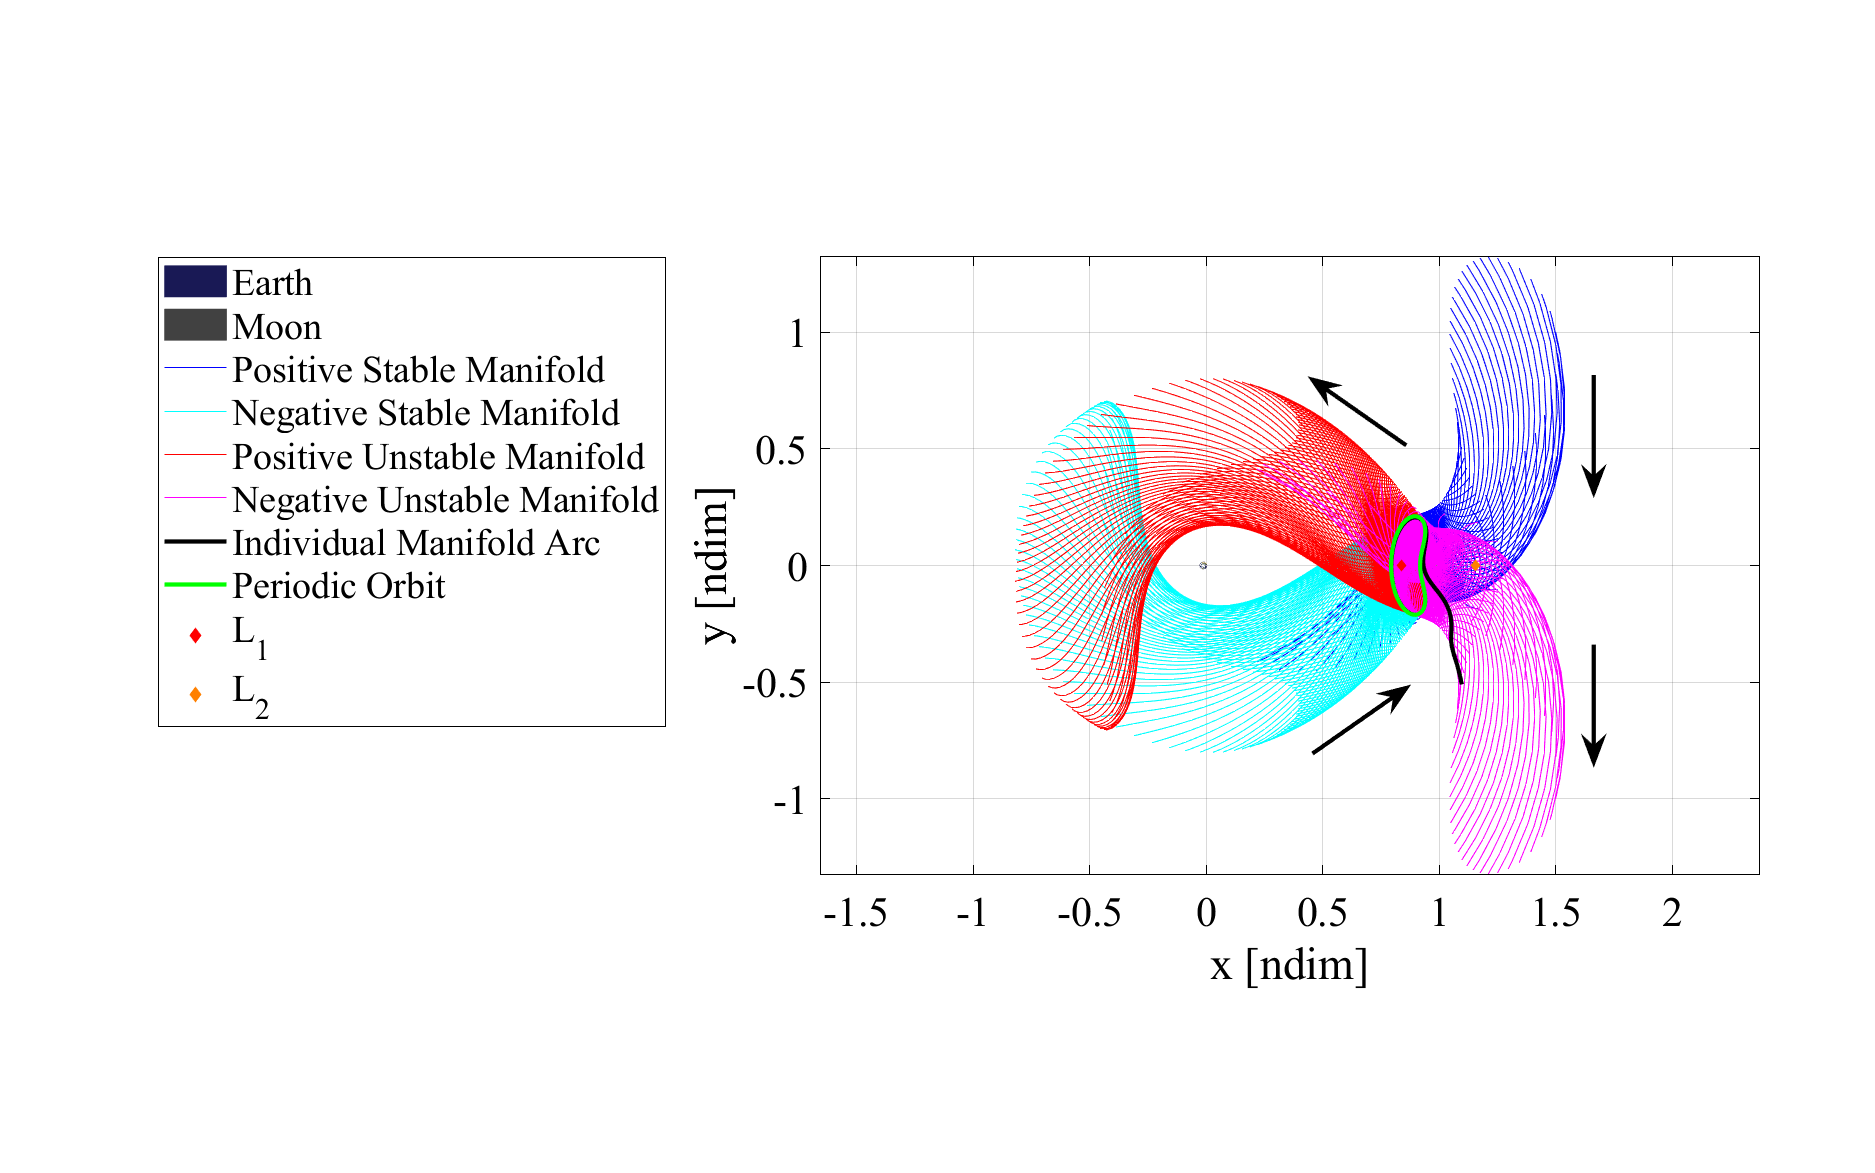
\includegraphics[width=0.9\textwidth]{figures/LyapunovManifold.pdf}
    \caption{Earth-Moon $L_{1}$ Lyapunov Manifolds ($C=3.05$).}
    \label{fig:LyapunovManifold}
\end{figure}

\begin{figure}[ht]
    \centering
    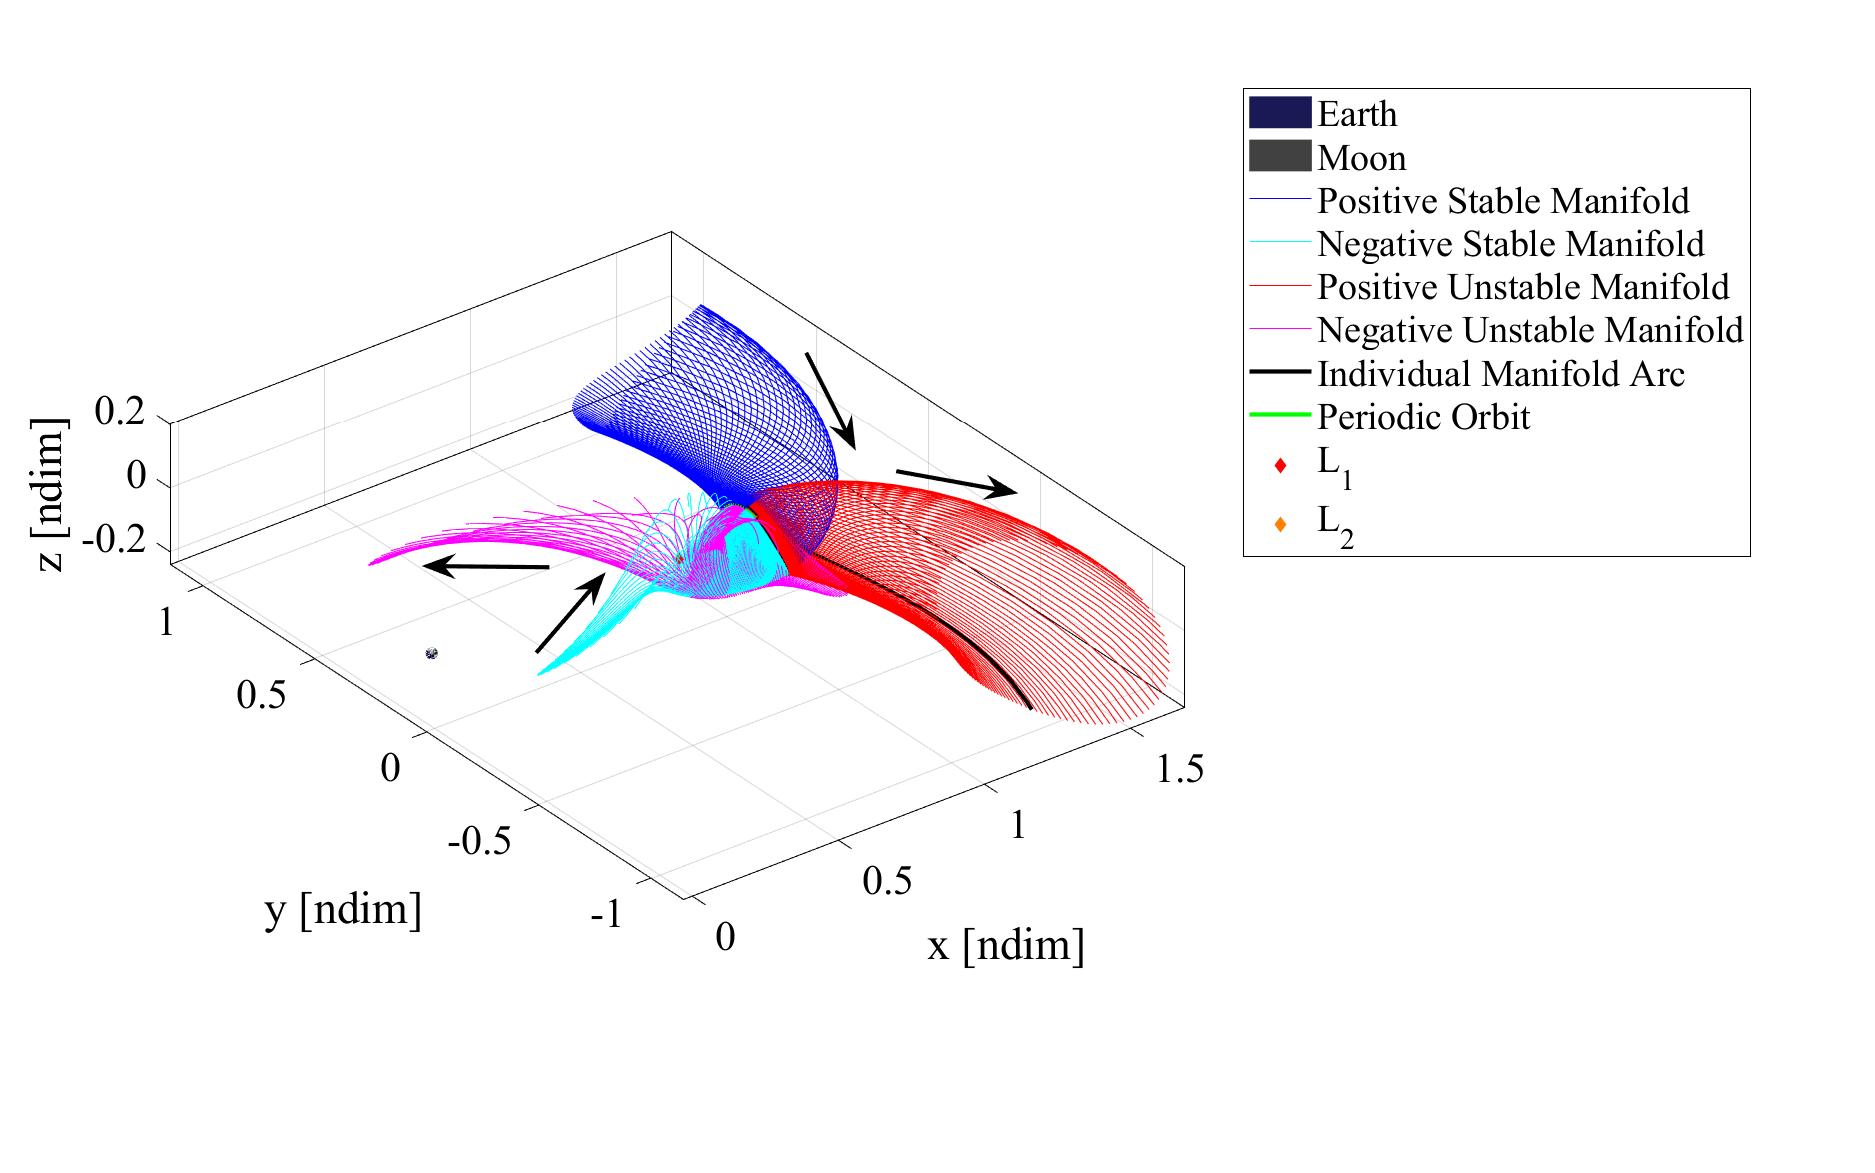
\includegraphics[width=0.9\textwidth]{figures/HaloManifold.pdf}
    \caption{Earth-Moon $L_{2}$ Halo Manifolds ($C=3.08$).}
    \label{fig:haloManifold}
\end{figure}

Since manifolds asymptotically arrive at/depart from their orbit, even with a reasonable step-off
distance, they can take a long time to depart from the orbit vicinity. Under higher-fidelity
dynamics, this period of time would be eliminated from the mission design, so it would be useful to
have a metric to determine when the manifold has departed the orbit vicinity. In this
investigation, the momentum integral, or more specifically the momentum integral difference, is
used to indicate orbit departure:
\begin{equation}
    MI=\int_{t_{0}}^{t}(x\xdot+y\ydot+z\zdot)d\tau,
    \label{eq:momentumintegral}
\end{equation}
where all of the values are nondimensional. Starting from $MI_{0}=0$ at the step-off location, the
momentum integral is calculated for both the orbit and the manifold arc and the difference between
the two values measures the similarity of the two trajectories:
\begin{equation}
    \Delta MI=|MI-MI_{\Gamma}|.
    \label{eq:momentumdifference}
\end{equation}
Once $\Delta MI$ has reached a threshold value (determined for each system), the trajectory is
considered departed from the orbit\cite{Guzzetti:2017}. \cref{tab:manifoldValues} shows the
threshold values chosen for each system in this investigation.

\begin{table}[ht]
    \centering
    \caption{Manifold-related values of relevant CR3BP systems.}
    \begin{tabular}{|c|c|c|}
        \hline
        \textbf{CR3BP System}   &   \boldmath$d$ \textbf{[km]}  &   \boldmath$\Delta MI$    \\  \hline
        Earth-Moon              &   $25$                        &   $1\times10^{-3}$        \\  \hline
        Sun-Earth               &   $1000$                      &   $5\times10^{-5}$        \\  \hline
        Sun-Mars                &   $1000$                      &   $1\times10^{-5}$        \\  \hline
    \end{tabular}
    \label{tab:manifoldValues}
\end{table}
